\documentclass[acmsmall,screen]{acmart}
% Packages and definitions for the acmart (ACM Computing Surveys) build.
% acmart already loads amsmath, xcolor, graphicx, hyperref, natbib and booktabs; layout and fonts are
% fixed by the class and are not changed here.
\usepackage{tabularx,multirow,array}
\usepackage{subcaption}
\usepackage{enumitem}
\usepackage[most]{tcolorbox}
\usepackage{adjustbox}
\usepackage{tikz}
\usetikzlibrary{arrows.meta,positioning,fit,backgrounds,calc,shapes.geometric,shapes.misc,decorations.pathreplacing}
\usepackage[nameinlink,capitalise,noabbrev]{cleveref}

% Palette shared by all figures (six functional categories; validated for colour-vision deficiency,
% always paired with text labels).
\definecolor{encode}{HTML}{2A78D6}
\definecolor{anticipate}{HTML}{EB6834}
\definecolor{compute}{HTML}{1BAF7A}
\definecolor{provision}{HTML}{6250D6}
\definecolor{connect}{HTML}{E87BA4}
\definecolor{assure}{HTML}{008300}
\definecolor{gapcolor}{HTML}{B03A2E}

\setlist{itemsep=1pt,topsep=3pt}
\graphicspath{{figures/}}

\newtcolorbox{openproblemsbox}{breakable,enhanced,colback=gapcolor!3,colframe=gapcolor!65!black,
  boxrule=0.6pt,arc=1.5pt,fonttitle=\bfseries\sffamily\small,title={Open problems},
  left=5pt,right=5pt,top=3pt,bottom=3pt}
\newenvironment{openproblems}{\begin{openproblemsbox}\small\begin{enumerate}[label=\textbf{P\arabic*.},leftmargin=2em,itemsep=2pt]}{\end{enumerate}\end{openproblemsbox}}


\setcopyright{none}
\acmJournal{CSUR}
\acmYear{2026}

\begin{document}

\title{Networked Extended Reality since 2023: Closing the Loop between Network and Experience}

\author{Anonymous}
\affiliation{%
  \institution{To be completed}
  \city{}
  \country{To be completed}}

\begin{abstract}
Since 2023, networked extended reality (XR) has moved to standalone headsets that stream rendered frames,
avatars, point clouds and Gaussian splats over Wi-Fi and 5G-Advanced. This review covers what recent work
has built, measured and learned, with a focus on networking and quality of experience (QoE). User studies
agree that loss, jitter and stalls hurt more than tens of milliseconds of added delay, but nearly all of
them apply static impairments to one user or one pair. Measurements of commercial headsets and platforms
show that the application stack often sets what users see, and that standard XR traffic models
underestimate real demand. In the radio access, 5G-Advanced makes scheduling aware of video frames through
PDU sets, and network-assisted rate control, Wi-Fi~7 multi-link operation and robust mmWave beams follow
the same idea. In transport, L4S, Media over QUIC and selective forward error correction aim at frame
deadlines rather than throughput, while foveated, split and Gaussian-splat delivery adapt what is sent. We
group these approaches by the idea they share, state what each assumes, and show that capacity gains are
almost always counted in packet-delay budgets, not in validated QoE. We close with open research questions
on replaying real network dynamics to users, on who should own the rate control loop, and on group
experience.
\end{abstract}

\begin{CCSXML}
<ccs2012>
<concept><concept_id>10003033.10003106.10003113</concept_id><concept_desc>Networks~Mobile networks</concept_desc><concept_significance>500</concept_significance></concept>
<concept><concept_id>10003033.10003079</concept_id><concept_desc>Networks~Network performance evaluation</concept_desc><concept_significance>500</concept_significance></concept>
<concept><concept_id>10003120.10003121.10003124.10010866</concept_id><concept_desc>Human-centered computing~Virtual reality</concept_desc><concept_significance>300</concept_significance></concept>
</ccs2012>
\end{CCSXML}
\ccsdesc[500]{Networks~Mobile networks}
\ccsdesc[500]{Networks~Network performance evaluation}
\ccsdesc[300]{Human-centered computing~Virtual reality}

\keywords{extended reality, quality of experience, split rendering, 5G-Advanced, PDU set, Wi-Fi 7,
millimetre wave, L4S, Media over QUIC, volumetric video, Gaussian splatting, cloud VR gaming, social XR}

\maketitle

\section{Introduction}\label{sec:intro}

Networked extended reality (XR) changed shape after 2023. The standalone headset became the main client:
it tracks the user, renders what it can, and streams the rest from an edge or cloud renderer. Split
rendering moved from cables to Wi-Fi~6 and 7 and to 5G-Advanced, where 3GPP Releases 18 and 19 added the
first radio features designed around XR traffic \cite{W7164211432}. The content changed too.
Besides rendered frames and 360-degree video, systems now stream point clouds, avatars sent as keypoints
\cite{W4403981191}, and 3D Gaussian splats \cite{W4416477288}. The metaverse push added social sessions in
which several people share one scene and judge each other's delay.

These changes couple networking and quality of experience (QoE) more tightly than before. A frame is
useful only if it arrives before its display deadline, so the network decides whether an image appears,
not only how sharp it is. The headset hides head-rotation delay by reprojection, but it cannot hide a lost
frame, a frozen peer or a stalled scene. The coupling now also runs the other way. The radio can learn
which packets form one frame and how much each frame matters \cite{W4410582180}, and an application can be
told what rate the cell can carry \cite{W7161282618}. \Cref{fig:loop} draws the resulting control loop.
Every mechanism in this review closes some part of it, and the question for each is whether the part it
closes is the one users perceive.

\begin{figure}[t]
\centering
\begin{adjustbox}{max width=\linewidth}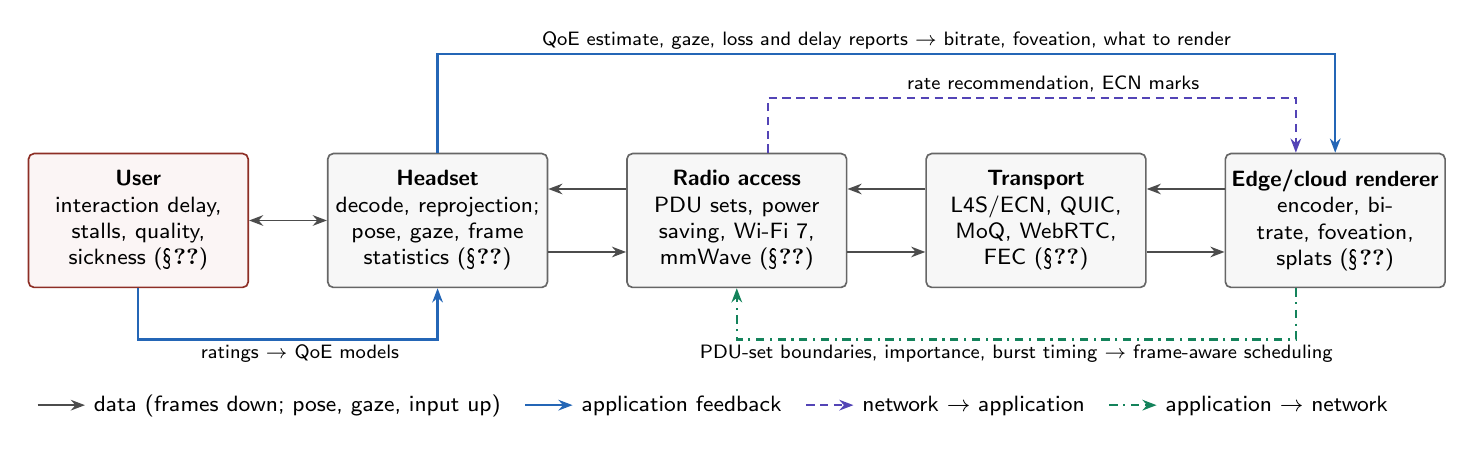
\begin{tikzpicture}[font=\sffamily\footnotesize,
  blk/.style={draw=black!60, fill=black!3, rounded corners=2pt, align=center, text width=2.65cm,
    minimum height=17mm, inner sep=2pt, line width=0.6pt},
  usr/.style={blk, draw=gapcolor!80!black, fill=gapcolor!5},
  data/.style={-{Stealth[length=1.8mm]}, line width=0.7pt, draw=black!70},
  app/.style={-{Stealth[length=1.8mm]}, line width=0.8pt, draw=encode!85!black},
  net/.style={-{Stealth[length=1.8mm]}, line width=0.8pt, draw=provision!85!black, densely dashed},
  aware/.style={-{Stealth[length=1.8mm]}, line width=0.8pt, draw=compute!75!black, dash dot},
  lab/.style={font=\sffamily\scriptsize, align=center, text=black, inner sep=1.5pt}]
\node[usr] (u) at (0,0)     {\textbf{User}\\interaction delay, stalls, quality, sickness (\S\ref{sec:qoe})};
\node[blk] (h) at (3.8,0)   {\textbf{Headset}\\decode, reprojection; pose, gaze, frame statistics (\S\ref{sec:measure})};
\node[blk] (a) at (7.6,0)   {\textbf{Radio access}\\PDU sets, power saving, \mbox{Wi-Fi~7}, mmWave (\S\ref{sec:radio})};
\node[blk] (t) at (11.4,0)  {\textbf{Transport}\\L4S/ECN, QUIC, MoQ, \mbox{WebRTC}, FEC (\S\ref{sec:transport})};
\node[blk] (r) at (15.2,0)  {\textbf{Edge/cloud renderer}\\encoder, bitrate, foveation, splats (\S\ref{sec:transport})};
% data plane: downlink above, uplink below
\foreach \x/\y in {r/t,t/a,a/h} \draw[data] ([yshift=4mm]\x.west) -- ([yshift=4mm]\y.east);
\foreach \x/\y in {h/a,a/t,t/r} \draw[data] ([yshift=-4mm]\x.east) -- ([yshift=-4mm]\y.west);
\draw[data, {Stealth[length=1.8mm]}-{Stealth[length=1.8mm]}] (u.east) -- (h.west);
% control loops
\draw[app] (h.north) -- ++(0,1.25) -| node[lab, pos=0.25, above] {QoE estimate, gaze, loss and delay reports
  $\rightarrow$ bitrate, foveation, what to render} (r.north);
\draw[net] ([xshift=4mm]a.north) -- ++(0,0.7) -| node[lab, pos=0.27, above] {rate recommendation, ECN marks} ([xshift=-5mm]r.north);
\draw[aware] ([xshift=-5mm]r.south) -- ++(0,-0.65) -| node[lab, pos=0.25, below] {PDU-set boundaries, importance, burst timing $\rightarrow$ frame-aware scheduling} (a.south);
\draw[app] (u.south) -- ++(0,-0.65) -| node[lab, pos=0.27, below] {ratings $\rightarrow$ QoE models} (h.south);
% legend
\node[lab, anchor=west, align=left, font=\sffamily\footnotesize] at (-1.35,-2.35) {%
  \tikz[baseline=-0.6ex]\draw[data] (0,0)--(0.6,0); data (frames down; pose, gaze, input up)\quad
  \tikz[baseline=-0.6ex]\draw[app] (0,0)--(0.6,0); application feedback\quad
  \tikz[baseline=-0.6ex]\draw[net] (0,0)--(0.6,0); network $\rightarrow$ application\quad
  \tikz[baseline=-0.6ex]\draw[aware] (0,0)--(0.6,0); application $\rightarrow$ network};
\end{tikzpicture}\end{adjustbox}
\caption{The QoE control loop of a networked XR session and the sections that discuss each part. The
application adapts to its own measurements, the network recommends rates or marks congestion, and the
application tells the network which packets form a frame. Only the path from users' ratings to QoE models
rests on user studies.}
\label{fig:loop}
\end{figure}

This review covers work published from 2023 to 2026 and follows the loop from the user outwards:
what users perceive (\cref{sec:qoe}), what measurements of real systems show (\cref{sec:measure}), the
radio access (\cref{sec:radio}), and transport and delivery (\cref{sec:transport}). \Cref{tab:families}
classifies the families of mechanisms, and \cref{sec:outlook} states open problems. Throughout, we
separate what is \emph{established} (measured on real systems or with users), what is \emph{contested},
and what is \emph{assumed}.

\section{What Users Experience}\label{sec:qoe}

\subsection{Loss and jitter outweigh delay}
Recent user studies agree on one ordering: loss, jitter and stalls hurt more than tens of milliseconds of
added delay. With Nvidia CloudXR and a first-person shooter (N=30), QoE fell at a round-trip time (RTT) of
75~ms or more, or at loss above 6\%; combined, 25~ms with 4\% loss was already harmful \cite{W4402156718}.
In a social XR application (N=28), RTT up to 77~ms had no significant effect, while loss above 2\% at
higher RTT did, and even jitter of one standard deviation degraded QoE at RTTs beyond 52~ms
\cite{W4415822410}. With a Quest~3 streaming over Air Link (N=16), loss harmed experience more than delay
across almost all measured aspects \cite{W4404916373}. In Rec Room and VRChat, the virtual environment
froze under loss but not under latency \cite{W4404103205}.

The ordering follows from how the headset splits latency. Reprojection serves head rotation locally, so
network delay reaches only \emph{interaction latency}: aiming, grabbing, or seeing a peer react. That
budget depends on timing structure, not on RTT alone. In split-rendered gaming, 90 and 120~fps tolerated
up to 6~ms of network delay before responsiveness suffered, and 60~fps was the better choice when delay
was high \cite{W4401943426}. The budget is therefore \emph{contested}: requirement statements still ask for
sub-20~ms end-to-end latency \cite{W7126117938}, while users of cloud and social XR tolerated RTTs near
75~ms. Cybersickness depends on content more than on the network: loss raised sickness in Beat Saber but lowered presence in Cubism \cite{W4404916373}, and at most 21\% of viewers
reported dizziness for point clouds in AR \cite{W4387831705}.

\subsection{Experience is social}
Multi-user sessions add effects no single-user study can show. In collaborative VR (20 participants in
pairs), users told impaired from unimpaired sessions but not latency from bursts, task time and sickness
scores did not change, and the user's role shaped perception \cite{W4392600587}. Impairments also raised synchronisation traffic four- to fivefold through retransmissions. Avatars
expose a fidelity trade-off. With 40 participants on Quest~Pro headsets, a light cartoon avatar gave the
highest QoE under impairment; a humanoid avatar that replicates facial expressions lost more under delay,
yet seeing a partner's face softened the loss \cite{W4415821547}. Standards lag behind: ITU-T leads in
modelling social aspects of QoE, but 3GPP, ITU-T and ETSI efforts remain fragmented and centred on system
metrics \cite{W4415822422}.

\subsection{Predicting experience}
Three families of models map what can be observed to what users would report.
\emph{Opinion-trained models} fit ratings from a lab study: cloud VR gaming models reached a Pearson
correlation of 0.93 \cite{W4400981668}, and regression models for a VR shooter a mean absolute error of 0.14 \cite{W4405935991}. Fed with real traces, the latter predicted a mean opinion
score (MOS) of only 2.5--3.0 over 4G and 5G against 4.2--4.4 over wired access. \emph{Content-quality
metrics} cover new media: colour PSNR correlated with point-cloud ratings at 0.84 \cite{W4387831705}, but
common metrics missed the effect of viewing behaviour on volumetric video \cite{W4386172458}.
\emph{Network-side estimators} infer QoE from what an operator sees, such as encrypted 360-degree traffic
over HTTPS and QUIC in 4G and 5G drive tests \cite{W4384158049} or QoS counters on an O-RAN testbed
\cite{W4389923869}, but are validated against application metrics, not users.

All three families inherit one study design: \emph{static impairments}. Emulators apply a constant RTT,
independent loss or a fixed jitter distribution to 16--40 participants, and real 4G and 5G measurements
enter only afterwards, as inputs to models fitted under constant conditions
\cite{W4405935991,W4415822410}. That thresholds learned this way hold under bursty, correlated wireless loss is \emph{assumed}.

\section{Measuring Real Systems}\label{sec:measure}

\subsection{Commercial headsets and platforms}
Measurements of commercial systems show that the application stack, not the link, often decides what
users see. On Apple Vision Pro, FaceTime sends a spatial persona over QUIC at about 0.7~Mbps; the bitrate
matches face and hand keypoints, not a mesh, which would need over 100~Mbps at 90~fps
\cite{W4403981191}. The same study found no rate adaptation: with the uplink capped at 0.7~Mbps the
persona disappeared. Servers were chosen near the session initiator, which gave RTTs above 100~ms within
the United States, and downlink traffic grew almost linearly from two to five users because servers
forward each persona. On a Quest~Pro, the old 2.4~GHz Wi-Fi~4 kept 99\% of samples at or above 65~Hz
against a 72~Hz target, while wireless offloading drained the battery 15\% faster than local rendering
\cite{W4362489903}. One 45-minute social VR session on Multiverse touched 87 service domains, and its time-critical state ran as UDP at about
30 packets per second upstream \cite{W4389609035}. Steam Link on a Quest~3 carries video and control in one
QUIC tunnel, with a bursty downlink and a periodic uplink; scene complexity set the mean throughput, the
player's style its variance \cite{W7160626692}.

\subsection{Access networks in practice}
In-situ tests expose interactions that link-level figures hide. One Wi-Fi~6 access point served three
headsets at up to 100~Mbps each with latency near 50~ms, but uplink OFDMA delayed tracking packets and
thus rendering \cite{W4396853623}. With Unity Render Streaming over Wi-Fi~6, the WebRTC pacer released
frames in 5.56~ms batches and added 6--21~ms of frame assembly delay although the RTT was 1.5~ms
\cite{W4391506055}. Cellular access trades direction: a 5G standalone edge setup gave a steadier downlink
and better mobility than Wi-Fi~6, but higher uplink latency on the control channel \cite{W4399563011}, and
a local 5G test network measured 3.4--4.1~ms one-way delay downlink against 6.4--14.8~ms uplink
\cite{W7126117938}. In these studies the uplink, which carries pose and input, was the weaker direction.

\subsection{Testing the traffic models}
The simulations in \cref{sec:radio} rest on traffic models, and measurements now test them. For cloud VR on
a Pico Neo~2, the 3GPP baseline underestimated the effective bitrate by 25\% \cite{W4399340506}. Frame
sizes in ALVR depend on head angular velocity, so a model that includes motion predicted them better
\cite{W4414539403}. Modern 6DoF gaming reached 251.9~Mbps and 120~Hz, beyond the fixed 50~Mbps and 60~Hz
many models assume \cite{W4411688686}, and cloud-rendered AR traces showed heavy-tailed packet sizes and
loss that is rare on average but arrives in bursts \cite{W7202080971}. Real XR traffic is larger, burstier and more motion-dependent than baseline models assume, so
the capacity figures of \cref{sec:radio} are likely optimistic.

\section{The Radio Access}\label{sec:radio}

The common idea of radio work since 2023 is to change the unit of service from the packet to the video
frame. A frame that misses its deadline is worthless even if most of its packets arrive. \Cref{tab:families} classifies the
resulting families together with those of \cref{sec:transport}.

\begin{table}[t]
\centering\footnotesize
\caption{Families of network and delivery mechanisms for XR since 2023, what they were evaluated on, and
whether users confirmed the gain. ``Proxy'' means a network or image metric stands in for QoE.}
\label{tab:families}
\setlength{\tabcolsep}{3.5pt}
\begin{tabularx}{\linewidth}{@{}>{\raggedright\arraybackslash}p{3.2cm}>{\raggedright\arraybackslash}X>{\raggedright\arraybackslash}p{3.0cm}>{\raggedright\arraybackslash}p{2.1cm}@{}}
\toprule
Family & Idea & Evaluated on & QoE validated?\\
\midrule
Frame-aware scheduling & Schedule PDU sets against a frame deadline & System-level simulation & No; PDB met\\
Coexistence and power & Limit interference; sleep between frames & System-level simulation & No\\
Network-assisted rate & Network recommends a rate & Simulation, testbed & No; outage\\
Wi-Fi~7 MLO, mmWave & Several links; beams that follow the head & Simulation, lab hardware & No; delay, loss\\
Early congestion signals & L4S/ECN, in-network dropping & Emulation, testbeds & Proxy; frame loss\\
QUIC and MoQ delivery & Streams, delivery timeouts & Emulation & Proxy; stalls\\
Selective protection & FEC on what matters, neural repair & Loss traces & Proxy; freezes\\
Perception-driven sending & Foveation, QoE-model encoding & Prototypes with users & Yes, small labs\\
Volumetric, splat delivery & Layered, progressive, shared content & Datasets, prototypes & Mostly proxy\\
\bottomrule
\end{tabularx}
\end{table}

\subsection{Making the radio frame-aware}
\emph{PDU sets} are the standard vehicle. 3GPP Release 18 defines a PDU set as the smallest group of
packets that carries one frame, together with its relative importance, and lets the radio network apply
QoS handling to it \cite{W4410582180}. Release 19 adds burst signalling, expedited transfer of
latency-critical content and guidance on importance values \cite{W7127418717}, plus radio features such
as latency-aware uplink prioritisation, delay status reports and uplink rate control through application
adaptation \cite{W7164211432}. \emph{Frame-aware schedulers} exploit this information. A PDU-set scheduler
raised XR capacity by up to 45\% at unchanged broadband throughput \cite{W4402156740}, and an uplink
least-slack-time scheduler gained 15\% capacity and cut XR packet delay by up to 33\% in a nine-cell dense
urban case \cite{W4406264804}.

\subsection{Coexistence and energy}
XR rarely has a cell to itself. Adding a 45~Mbps XR flow with a 10~ms packet delay budget (PDB) cost about
45~Mbps of broadband capacity \cite{W4385801627}, but interference from broadband users in other cells
removed about 80\% of XR capacity; restricting broadband throughput by about half restored it at a 20~ms
PDB \cite{W4387546593}. Power saving competes with delay: standardised and proposed sleep schemes saved
6--23\% of device energy without delaying traffic unacceptably \cite{W4406265335}.

\subsection{Telling the application what the network can carry}
A second family closes the loop from network to application (\cref{fig:loop}). NetXRate combines
core-network analytics with an O-RAN xApp to recommend rates, and cut outage by up to 96\% against
over-the-top adaptation in simulation \cite{W7161282618}. On a 4G O-RAN testbed, an xApp held VR latency
near its target and freed 15.8\% of resources for other users \cite{W4392175446}.

\subsection{Wi-Fi~7 and millimetre wave}
\emph{Multi-link operation} (MLO) in Wi-Fi~7 lets one device use several channels. In simulation, it
supported seven AR stations where a single link supported six, while policies that need simultaneous
access to all links suffered under contention \cite{W4376480829}; for the same total bandwidth, more and
narrower links gave lower delay than fewer wide ones \cite{W4412836976}. \emph{Millimetre wave} offers the
rates that uncompressed Quest~3 video would need (15.75--26.25~Gbps), yet tested hardware delivered
1.85--1.98~Gbps, and moderate head rotation at 45 degrees per second drove loss to 4.72\% in one
configuration \cite{W4401507876}. Dual-beam reception across coordinated access points improved reliability by up to 22.8\% on real head-motion traces \cite{W4409076649}.

These results share their assumptions: system-level simulation with 3GPP-style traffic, which
\cref{sec:measure} found too light, and a user counted as satisfied when enough packets meet the PDB. No
study has yet shown that frame-aware scheduling raises the QoE that \cref{sec:qoe} measured.

\section{Transport and Delivery}\label{sec:transport}

Above the radio the question is the same: deliver each frame before its deadline, and send less when the
path cannot.

\subsection{Earlier congestion signals}
Delay- and loss-based controllers react after a queue has formed, which is a frame too late for XR.
\emph{L4S} marks congestion before queues grow. In volumetric video conferencing, an L4S pipeline
converged on the available rate 45\% faster than Google Congestion Control (GCC) and lost no packets,
while the WebRTC baseline left 3\% of frames undecodable \cite{W4408870658}. \emph{Comparisons of
existing controllers} remain mixed: integrated into ALVR, GCC tracked the available rate closely with few
dropped frames, but only NADA held a fair share against loss-based flows \cite{W4415538381}.
\emph{In-network adaptation} moves the decision to the base station. Octopus lets senders overestimate
capacity and drops application-chosen packets at the cell, reporting 1.5--18$\times$ better performance
for standard and volumetric video \cite{W4401386494}.

\subsection{Transports with deadlines}
QUIC removes transport head-of-line blocking and offers unreliable datagrams. \emph{Media over QUIC} (MoQ)
adds delivery timeouts, which a point-cloud server used for implicit adaptation: clients with tight
latency targets received lower quality, relaxed ones higher quality \cite{W4417496773}. WebRTC keeps its
strengths for groups: through a selective forwarding unit, volumetric video adapted to user movement 13\%
and 36\% faster than over TCP at 5 and 10~ms of network latency \cite{W7151958829}. Which transport suits
interactive XR is still \emph{contested}.

\Cref{sec:qoe} showed that loss, not delay, drives QoE, yet a retransmission costs a frame time.
\emph{Selective protection} spends redundancy where it matters. ReVo applies forward error correction (FEC)
to critical colour and depth content and repairs the rest with a neural module, cutting freezes by up to
95.7\% on real loss traces \cite{W7159678172}. A hybrid broadcast--unicast design masked typical wireless
loss with 15\% FEC overhead while keeping volumetric latency under 40~ms \cite{W4415933998}.

\subsection{Adapting what is rendered and sent}
\emph{Application-layer rate adaptation} is the oldest loop and still effective: over Wi-Fi, a
network-aware bitrate algorithm for ALVR adapted to contention and mobility \cite{W4405014964}.
\emph{Perception-driven sending} lets the user decide what to send, and it is the one family validated
with users. Dynamic foveation driven by streamed gaze added 0.60 MOS over static foveation while saving
9.81\% bitrate in cloud VR gaming \cite{W4377981508}, and EyeNexus adapted the foveal region to bandwidth
and cut latency by up to 70.9\% \cite{W4416659623}. Encoding settings driven by a learned QoE model raised
interaction quality by 1.20 MOS \cite{W4400981668}. \emph{Split decisions} move work between device and
edge: RenderFusion switches objects between local and remote rendering using a perceptual study of
latency \cite{W4389296467}.

\subsection{Volumetric and Gaussian-splat delivery}
Volumetric content turns the trade-off between bandwidth and latency into one between compression and
latency. In VR2Gather, compression cut bandwidth by more than 90\% but raised latency to 278.7~ms, and
DASH delivery reached 562~ms against 87.4~ms over TCP \cite{W4362496249}. MuV2 served over 30 untethered devices from
one access point by mixing direct volumetric streaming with remote rendering \cite{W4399121637}. Gaussian
splats bring compact, progressive formats: V\textsuperscript{3} streams about 0.5~MB per frame and renders
at 27~fps on a phone \cite{W4404525293}, Vega reaches 30~fps on smartphones by prioritising important
objects \cite{W4416477288}, and TIGAS renders splats remotely and streams 2D views over QUIC
\cite{W7160906632}. These systems report PSNR, SSIM and frame rate; none of them reports a networked user
study.

\section{Open Problems and Conclusion}\label{sec:outlook}

The loop in \cref{fig:loop} is now closed at every layer, but each layer closes it against its own
metric: the radio against delay budgets, transport against frame loss, the renderer against image
quality. Five questions would join the parts.

\begin{openproblems}
\item \textbf{Do QoE thresholds survive real network dynamics?} Every user study in \cref{sec:qoe} applied
  static delay, independent loss or fixed jitter, while measured wireless loss arrives in bursts
  \cite{W7202080971}. Replaying recorded Wi-Fi and 5G traces to participants would show whether the
  tolerance of 75--77~ms RTT and the dominance of loss still hold.
\item \textbf{Does frame-aware scheduling raise QoE?} Frame-aware schedulers report 15--45\% more capacity
  \cite{W4402156740,W4406264804}, counted as packets that meet a PDB under traffic models that
  underestimate real demand \cite{W4399340506}. A testbed that couples such a scheduler to a headset and a
  QoE model would test whether capacity gains are experience gains.
\item \textbf{Who should own the rate?} Network recommendations \cite{W7161282618}, Release-19 uplink rate
  control \cite{W7164211432}, L4S marks \cite{W4408870658} and application bitrate adaptation
  \cite{W4405014964} can all act on one flow. Their joint stability, fairness and response time are
  unstudied.
\item \textbf{What is group QoE?} Social studies test pairs \cite{W4392600587,W4415821547}, while
  platforms serve five or more users through forwarding servers \cite{W4403981191}. How delay assigned to
  one member changes the experience of the others, and how to share impairments fairly, is unknown.
\item \textbf{Which representation for which link?} Point clouds, keypoint avatars, Gaussian splats and
  remotely rendered video trade bandwidth, device computation and latency differently, but each is
  evaluated alone and on image metrics \cite{W4404525293,W4416477288,W7160906632}. A common user-facing
  benchmark over the same network traces is missing.
\end{openproblems}

Since 2023, networked XR has gained frame-aware radios, earlier congestion signals, transports with
deadlines and content built for adaptation, while users have shown that reliability matters more than the
last tens of milliseconds. The next step is to judge each mechanism by the experience it produces under
real network dynamics, alone and in groups.


\bibliographystyle{ACM-Reference-Format}
\bibliography{data/references}
\end{document}
